\documentclass[spanish]{article}

\usepackage{nips13submit_e,times}
\nipsfinaltrue

\usepackage[spanish,es-nodecimaldot, es-tabla]{babel}
\usepackage[utf8]{inputenc}


% adds hyper links inside the generated pdf file
\usepackage[final]{hyperref}
\usepackage{graphicx}
\usepackage{caption}
% \usepackage{multirow}
% \usepackage{algorithm,algpseudocode}
\usepackage{subfigure}

\setlength{\marginparwidth}{2cm}
\usepackage{subfig}
\usepackage{amsmath}
% \usepackage{listings}
% \lstset{ %
%     basicstyle=\footnotesize,       % the size of the fonts that are used for the code
%     numbers=left,                   % where to put the line-numbers
%     numberstyle=\footnotesize,      % the size of the fonts that are used for the line-numbers
%     stepnumber=1,                   % the step between two line-numbers. If it is 1 each line will be numbered
%     numbersep=5pt,                  % how far the line-numbers are from the code
%     showspaces=false,               % show spaces adding particular underscores
%     showstringspaces=false,         % underline spaces within strings
%     showtabs=false,                 % show tabs within strings adding particular underscores
%     frame=single,           % adds a frame around the code
%     tabsize=2,          % sets default tabsize to 2 spaces
%     captionpos=b,           % sets the caption-position to bottom
%     breaklines=true,        % sets automatic line breaking
%     breakatwhitespace=false,    % sets if automatic breaks should only happen at whitespace
%     escapeinside={\%*}{*)}          % if you want to add a comment within your code
% }
\usepackage{booktabs}
\usepackage{todonotes}

\newcommand\tab[1][1cm]{\hspace*{#1}}

% Load the package
%\usepackage[acronym]{glossaries}

% Generate the glossary
%\makeglossaries
%\input{acronyms}

\title{Robótica Inteligente \\ \small Práctica final: Mapeado láser}

\author{
        David Revillas \\
        \texttt{drevillas002@ikasle.ehu.eus}
        \and
        \textbf{Mónica Rampérez} \\
        \texttt{mramperez001@ikasle.ehu.eus}
}

% \definecolor{darkgreen}{rgb}{0,0.5,0}
% \definecolor{lightgray}{rgb}{0.95,0.95,0.95}
% \definecolor{gray}{rgb}{0.65,0.65,0.65}
% \lstset{basicstyle=\footnotesize\ttfamily,
%                 keywordstyle=\color{darkgreen}\bfseries,
%                 %identifierstyle=\color{blue},
%                 commentstyle=\color{gray},
%                 stringstyle=\ttfamily,
%                 showstringspaces=false,
%                 tabsize=2,
%                 backgroundcolor=\color{lightgray},
%                 literate=
%                 {á}{{\'a}}1 {é}{{\'e}}1 {í}{{\'i}}1 {ó}{{\'o}}1 {ú}{{\'u}}1
%                 {Á}{{\'A}}1 {É}{{\'E}}1 {Í}{{\'I}}1 {Ó}{{\'O}}1 {Ú}{{\'U}}1
%                 {à}{{\`a}}1 {è}{{\`e}}1 {ì}{{\`i}}1 {ò}{{\`o}}1 {ù}{{\`u}}1
%                 {À}{{\`A}}1 {È}{{\'E}}1 {Ì}{{\`I}}1 {Ò}{{\`O}}1 {Ù}{{\`U}}1
%                 {ä}{{\"a}}1 {ë}{{\"e}}1 {ï}{{\"i}}1 {ö}{{\"o}}1 {ü}{{\"u}}1
%                 {Ä}{{\"A}}1 {Ë}{{\"E}}1 {Ï}{{\"I}}1 {Ö}{{\"O}}1 {Ü}{{\"U}}1
%                 {â}{{\^a}}1 {ê}{{\^e}}1 {î}{{\^i}}1 {ô}{{\^o}}1 {û}{{\^u}}1
%                 {Â}{{\^A}}1 {Ê}{{\^E}}1 {Î}{{\^I}}1 {Ô}{{\^O}}1 {Û}{{\^U}}1
%                 {Ã}{{\~A}}1 {ã}{{\~a}}1 {Õ}{{\~O}}1 {õ}{{\~o}}1
%                 {œ}{{\oe}}1 {Œ}{{\OE}}1 {æ}{{\ae}}1 {Æ}{{\AE}}1 {ß}{{\ss}}1
%                 {ű}{{\H{u}}}1 {Ű}{{\H{U}}}1 {ő}{{\H{o}}}1 {Ő}{{\H{O}}}1
%                 {ç}{{\c c}}1 {Ç}{{\c C}}1 {ø}{{\o}}1 {å}{{\r a}}1 {Å}{{\r A}}1
%                 {€}{{\euro}}1 {£}{{\pounds}}1 {«}{{\guillemotleft}}1
%                 {»}{{\guillemotright}}1 {ñ}{{\~n}}1 {Ñ}{{\~N}}1 {¿}{{?`}}1
% }

% \DeclareMathOperator*{\argmax}{arg\,max}

\begin{document}

\maketitle

\begin{abstract}
    El objetivo de esta práctica final es el de construir un mapa del entorno mientras se teleopera el robot a través del teclado utilizando información de odometría.
\end{abstract}

\pagenumbering{gobble}
%\tableofcontents
%\newpage
\pagenumbering{arabic}

\section{Introducción}

En esta práctica final se pretende desarrollar un módulo que permita construir un mapa del entorno mientras se teleopera el robot a través del teclado. Para ello, se necesita proyectar las lecturas del láser en el espacio de coordenadas global en el que se mueve el robot, haciendo uso de la odometría.

\subsection{Análisis del problema}

La idea es dibujar un mapa de puntos del entorno utilizando la información recibida por la parte delantera del escáner láser del robot. Para ello, será necesario proyectar los puntos detectados por el lídar teniendo en cuenta la posición del robot en cada momento, utilizando su odometría. Además, para que el mapeado del entorno sea completo, se podrá mover el robot de manera teleoperada, permitiendo que llegue a todos los lugares necesarios para completar el mapa.

\section{Estrategia utilizada}

\subsection{Descripción del \emph{Turtlebot}}

El robot utilizado en esta práctica es un \textit{Turtlebot} con lídar. Este escáner permite obtener un nube de puntos en 360º mapeándolos de la forma indicada en los ejes de la Figura \ref{fig:robot}.

\begin{figure}[!ht]
    \centering
    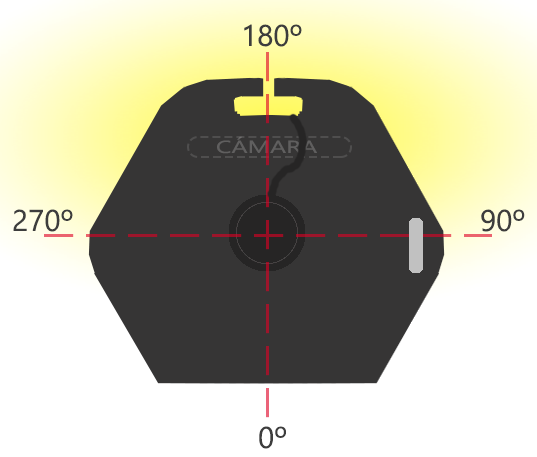
\includegraphics[scale=0.35]{images/robot.png}
    \caption{Esquema del robot \textit{Turtlebot}.}
    \label{fig:robot}
\end{figure}


\subsection{\emph{Topics} utilizados}
Para resolver esta práctica, la primera tarea es obtener la información del entorno. Nuestro robot \textit{Turtlebot} está provisto de un dispositivo lídar que permite obtener un nube de puntos en 360º, aunque en este caso sólo nos interesa utilizar los 180º que comprenden la parte delantera, como se indica en la Figura \ref{fig:robot}. Por tanto, utilizaremos la información recibida entre los 90º y los 270º. Esta nube de puntos la proporciona el \emph{topic} \texttt{scan} correspondiente al lídar, el cuál implementa el formato de mensaje \texttt{sensor\_msgs::LaserScan} con lo siguientes datos:


   \texttt{std\_msgs/Header header} 
\\ \tab \texttt{uint32 seq}
\\ \tab \texttt{time stamp} 

 \texttt{string frame\_id} 
 
 \texttt{float32 angle\_min} 
 
 \texttt{float32 angle\_max} 
 
 \texttt{float32 angle\_increment} 
 
 \texttt{float32 time\_increment} 
 
 \texttt{float32 scan\_time} 
 
 \texttt{float32 range\_min} 
 
 \texttt{float32 range\_max} 
 
 \texttt{float32[] ranges} 
 
 \texttt{float32[] intensities} 


Como vemos, el escáner proporciona gran cantidad de información, aunque los datos que realmente nos van a ser útiles en esta tarea se encuentran en el array \texttt{float32[] ranges}, que indica la distancia a la que se encuentra cada punto detectado para cada uno de los ángulos. De esta manera, la suscripción a este \emph{topic} nos permite conocer la situación del robot con el entorno prácticamente en tiempo real. 

Desde el \textit{topic} de odometría obtenemos la siguiente información del mensaje \texttt{nav\_msgs/Odometry}:
 
 \texttt{Header header}
 
 \texttt{string child\_frame\_id}
 
\texttt{geometry\_msgs/PoseWithCovariance pose}
 
 \texttt{geometry\_msgs/TwistWithCovariance twist}
 
Utilizaremos la información de \texttt{pose} para conocer la posición y la rotación del robot.

Por último, en este caso, para aplicar la velocidad de movimiento al robot, se utiliza el modulo \textit{teleop} previamente implementado.


\subsection{Mapeado del entorno}

Gracias a la odometría podemos conocer en cada momento las posiciones $x_r$ e $y_r$ del robot, así como su ángulo de orientación $\theta_r$.

Además, para cada uno de los 180 puntos detectados por el láser, tenemos la información de la distancia $I$ a la que se ha detectado y el ángulo $\theta_l$ al que corresponde.

Hemos establecido un umbral de 5 metros para dibujar sólo aquellos puntos que se detecten por debajo de esa distancia y así, con esta información es posible proyectar cada punto detectado en el mapa.

\[x_m = x_r + I*cos(\theta_r + \theta_l)\]
\[y_m = y_r + I*sin(\theta_r + \theta_l)\]

De esta manera, para cada instante de tiempo obtenemos las coordenadas de cada punto $x_m, y_m$ a dibujar en el mapa, como se muestra en la Figura \ref{fig:map_pasillo}.

\begin{figure}[!ht]
\centering
    \subfigure[]{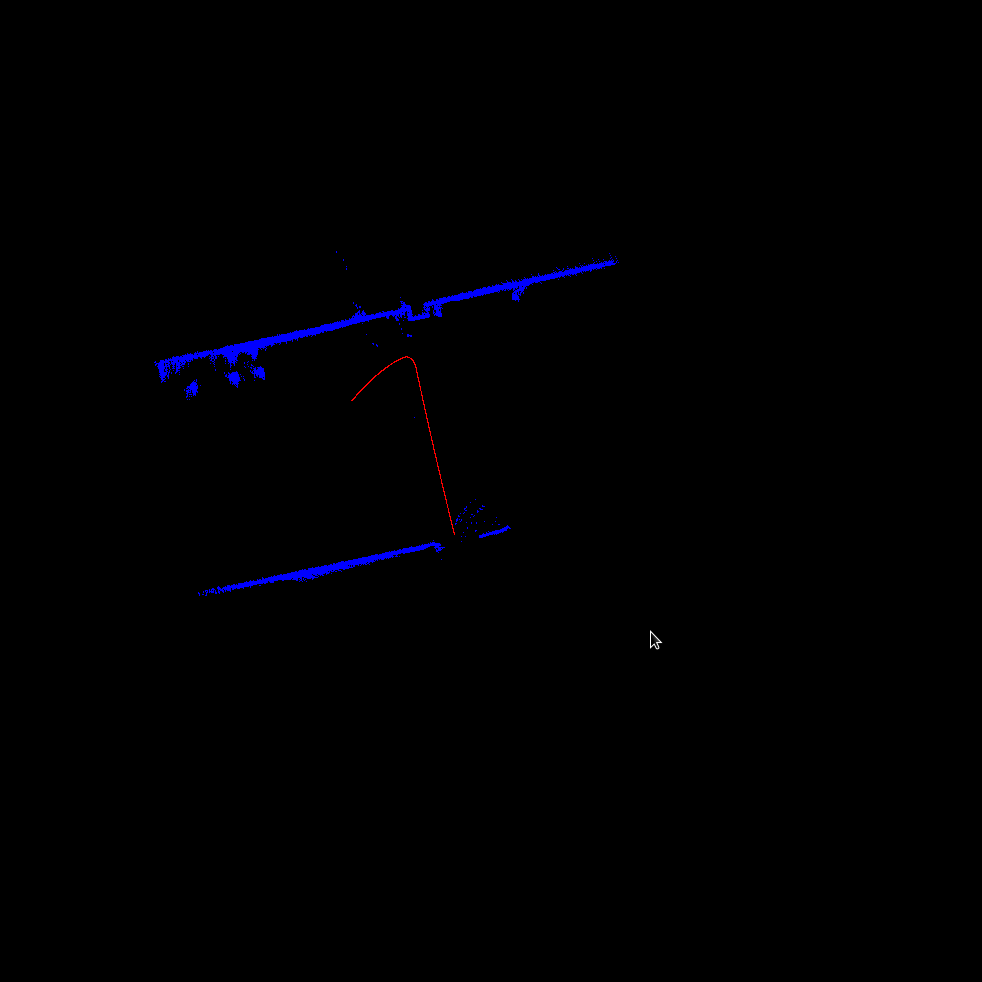
\includegraphics[width=45mm]{images/1.png}}
    \subfigure[]{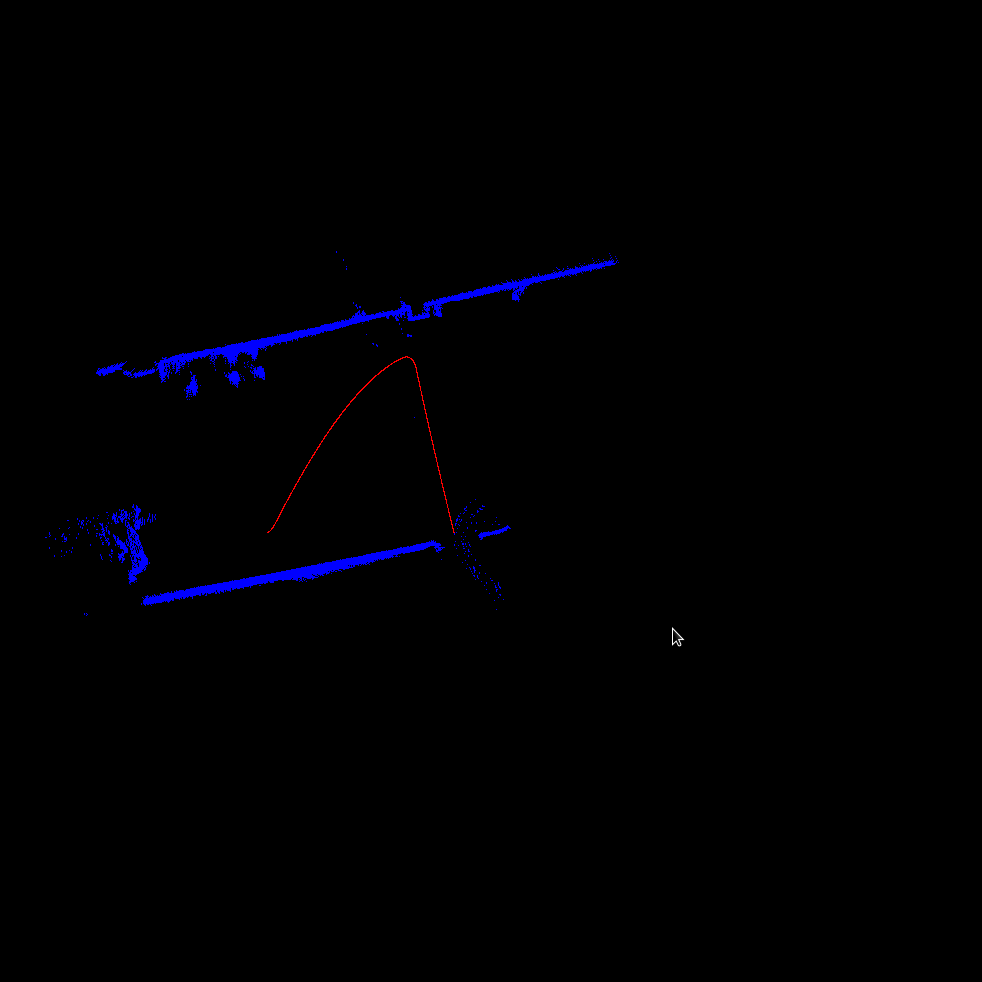
\includegraphics[width=45mm]{images/3.png}}
    \subfigure[]{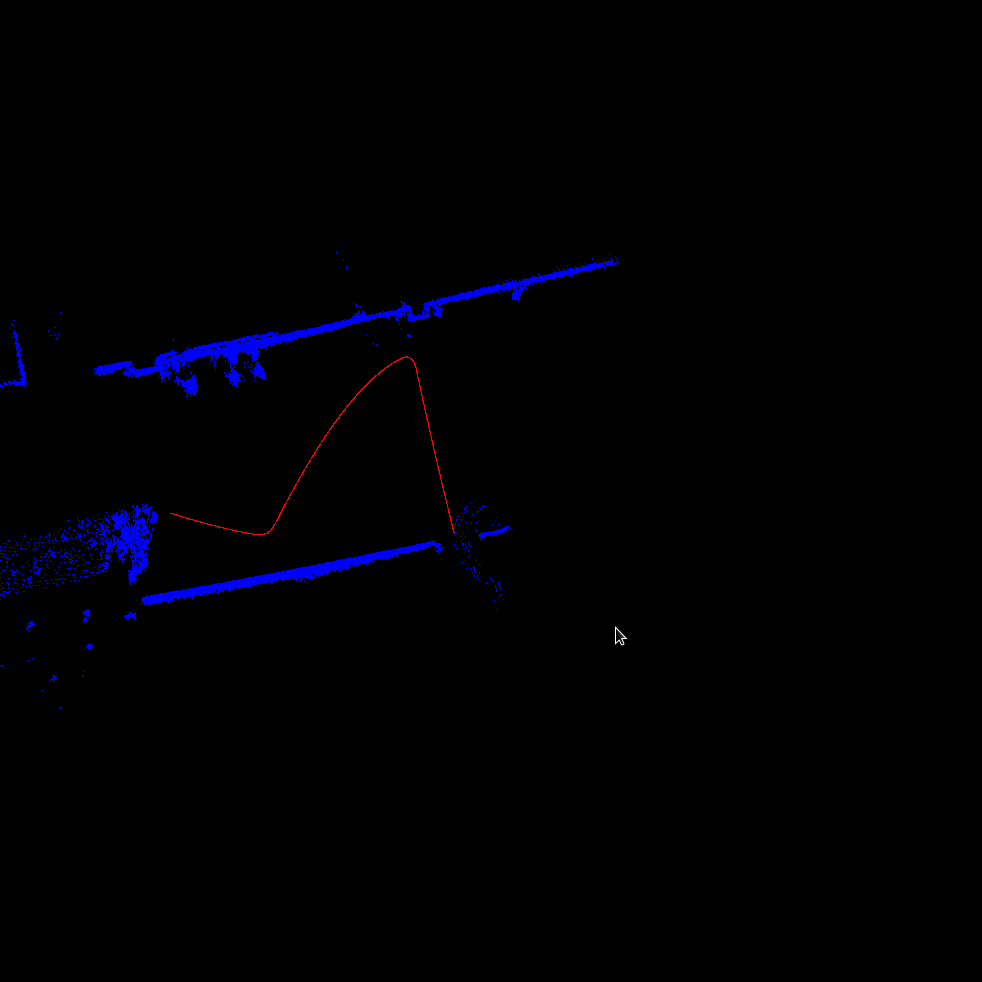
\includegraphics[width=45mm]{images/4.png}}
    \caption{Construcción progresiva del mapa del pasillo. A la izquierda de cada imagen, se encontrarían la escaleras, a la derecha, el laboratorio de los otros compañeros y en el punto de partida, la salida de nuestro laboratorio.} \label{fig:map_pasillo}
\end{figure}


\section{Evaluación del comportamiento}

Se ha probado a construir tanto el mapa del entorno de la clase como el del pasillo, con éxito en ambos casos. Sin embargo, es notable que los movimientos muy veloces y los giros rápidos provocan errores considerables que quedan reflejados en el dibujo del mapa.

En la Figura \ref{fig:clase} se observa una de las pruebas realizadas para el construir el mapa de la clase.

\begin{figure}[h]
    \centering
    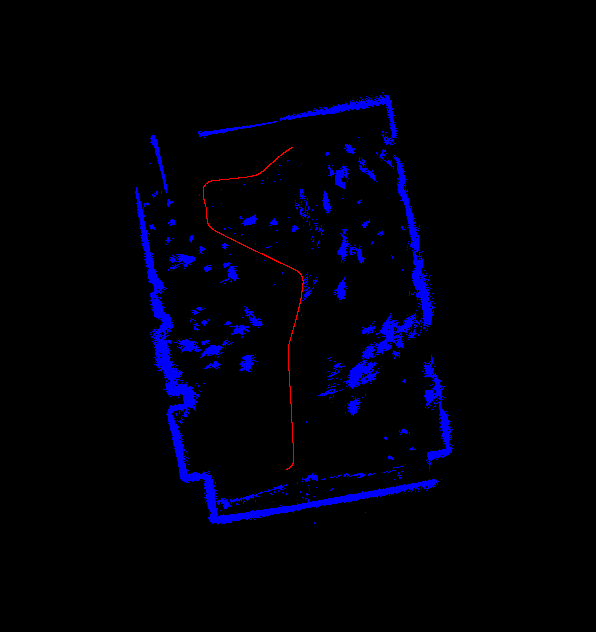
\includegraphics[scale=0.35]{images/mapa_clase.png}
    \caption{Mapa de la clase. La esquina superior izquierda correspondería a la entrada de la misma.}
    \label{fig:clase}
\end{figure}
\section{Extras}

\subsection{Sorteo de obstáculos}

Aunque no se trate de una mejora en sí del proceso de mapeado, se ha conseguido unir el módulo de sorteo de obstáculos, desarrollado en la primera práctica, junto al módulo implementado. Es por ello que la trayectoria que se muestra en la Figura \ref{fig:clase} resulta tan suave. De esta manera evitamos los saltos bruscos de velocidad y movimiento ocasionados por el módulo de \emph{teleop}.

\subsection{Difuminado}

Sólo por diversión, implementamos un difuminado de la imagen entre las líneas 193 y 198 del fichero \texttt{mapping.cpp}. En la implementación original, el callback \texttt{processOdom} actualiza la variable global \texttt{cv::Mat mymap} coloreando la matriz con datos de tipo \texttt{cv::Vec3b}, es decir, coloreando un píxel en rojo en la posición actual del \emph{turtlebot} y un píxel azul con el obstáculo localizado mediante el lídar. Sin embargo, esta implementación no hace más que ir añadiendo color indefinidamente a la matriz.

Nuestra implementación proponía reducir esos valores de manera constante mientras el escaneado del lídar no volviera a detectar el mismo obstáculo, concretamente, sustrayendo el vector \texttt{cv::Vec3b(12, 0, 1)} a cada elemento de la matriz, lo que supone que aproximadamente en $255 / 12 \approx 21 $ llamadas consecutivas a la función, un píxel que en cierto momento se hubiera detectado como obstáculo (elemento establecido como \texttt{cv::Vec3b(255, 0, 0)} en la matriz), en la llamada 22 desaparecería de la imagen. De manera similar para la trayectoria seguida por el robot, pero esta vez durante 255 llamadas. 

De esta manera, obtenemos un desvanecimiento de imágenes antiguas de forma progresiva, como se observa en la Figura \ref{fig:difuminado}. Se puede apreciar el desvanecimiento de la trayectoria roja, y más sutilmente, los obstáculos azules.

\begin{figure}[!ht]
    \centering
    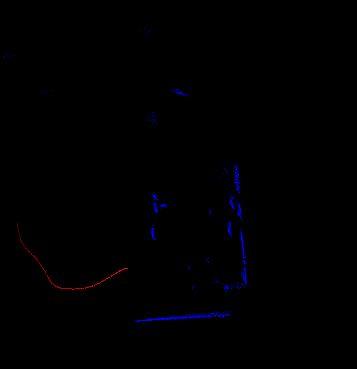
\includegraphics[scale=0.75]{images/difuminado.png}
    \caption{Resultado tras el difuminado aplicado en cada llamada a \texttt{processOdom}.}
    \label{fig:difuminado}
\end{figure}

\end{document}
